\documentclass[10pt,a4paper]{article}
\usepackage[utf8x]{inputenc}
\usepackage[T1]{fontenc}
%\usepackage{stringenc} % for grffile
\usepackage{ucs}
\usepackage{amsthm} %numéroter les questions
\usepackage[english]{babel}
\usepackage{datetime}
\usepackage{xspace} % typographie IN
\usepackage{hyperref}% hyperliens
\usepackage[all]{hypcap} %lien pointe en haut des figures
\usepackage[english]{varioref} %voir x p y
\usepackage{fancyhdr}% en têtes
%\input cyracc.def
\usepackage[]{graphicx} %include pictures
%\usepackage[encoding,inputencoding=utf8,filenameencoding=utf8]{grffile}
%\usepackage[extendedchars,inputencoding=latin1,filenameencoding=latin1]{grffile}
\usepackage[siunitx ]{circuitikz}
\usepackage{gnuplottex}
\usepackage{ifthen}
\graphicspath{{./figures/}}
%\usepackage{array}
\usepackage{amsmath}
\usepackage[]{xcolor}
\usepackage{tikz}
\usepackage{tikz-timing}
\usetikzlibrary{scopes}
\usetikzlibrary{backgrounds}
\usepackage{listings}
\usepackage{enumitem}
\usepackage[top=1 in, bottom=1 in, left=1.3 in, right=1 in]{geometry} % Yeah, that's bad to play with margins
\usepackage[]{pdfpages}
\usepackage{pdflscape}
\usepackage[]{attachfile}
%\usepackage{colortbl}
%\usepackage{multirow}
\usepackage{booktabs}
\usepackage{makecell}
\usepackage[ ]{subfig}
%\usepackage{rotating}
\usepackage{upgreek}

\newdateformat{mydate}{2017--2018}%hack pour remplacer \THEYEAR

%cyr
%\newcommand\textcyr[1]{{\fontencoding{OT2}\fontfamily{wncyr}\selectfont #1}}


\newboolean{corrige}
%\setboolean{corrige}{true}%corrigé
\setboolean{corrige}{false}% pas de corrigé

\newboolean{annexes}
%\setboolean{annexes}{true}%annexes
\setboolean{annexes}{false}% pas de annexes

\newboolean{mos}
%\setboolean{mos}{true}%annexes
\setboolean{mos}{false}% pas de annexes

\usepackage{aeguill} %guillemets

%% fancy header & foot
\pagestyle{fancy}
\lhead{[ELEC-H-410] Real-Time systems Labo n° 2: \uCOSII}
\rhead{\mydate\today\\ page \thepage}
\chead{\ifthenelse{\boolean{corrige}}{Corrigé}{}}
\cfoot{}
%%

\pdfinfo{
/Author (Yannick Allard - Raoul Sommeillier - Ken Hasselmann, ULB -- BEAMS)
/Title (Labo n° 2 ELEC-H-410, uCOS-II)
/ModDate (D:\pdfdate)
}

\hypersetup{
pdftitle={Labo n° 2 [ELEC-H-410] Real-Time systems},
pdfauthor={Yannick Allard - Raoul Sommeillier - Ken Hasselmann, ©2014-17 ULB - BEAMS  },
pdfsubject={uCOS-II}
}

\theoremstyle{definition}% questions pas en italique
\newtheorem{E}{\color{blue}Exercise}[] % numéroter les questions [section] ou non []

\newcommand{\reponse}[1]{% pour intégrer une réponse : \reponse{texte} : sera inclus si \boolean{corrige}
	\ifthenelse {\boolean{corrige}} {\paragraph{Réponse :} #1} {}
 }

\newcommand{\addcontentslinenono}[4]{\addtocontents{#1}{\protect\contentsline{#2}{#3}{#4}{}}}

\newcommand{\on}[1]{\operatorname{#1}}

\newcommand{\reg}[1]{\texttt{reg#1}}

\newcommand{\uCOSII}{$\upmu$C/OS-II}

\newcommand{\kw}[1]{\texttt{#1}}

\setlength{\parskip}{1ex plus .5ex minus .5ex} % espacement entre paragraphes
\setlength{\parindent}{0 ex plus 0ex minus 0 ex} % retrait en début de §

\def\labelitemi{--}
\setlist{parsep=0pt,itemsep=0pt,style=standard,leftmargin=\parindent, align=left} % pas d'espace prohibitif entre les items
\setlist{nolistsep}

\newcolumntype{C}[1]{>{\centering\let\newline\\\arraybackslash\hspace{0pt}}m{#1}}

%\setlength{\tabcolsep}{0pt} %no extra space in cells to keep constant tabular width

\date{\vspace{-1cm}\mydate\today}
\title{\vspace{-2cm} Labo n° 2\\ Real-Time systems [ELEC-H-410]\\ Sharing resources under \uCOSII~\ifthenelse{\boolean{corrige}}{~\\Corrigé}{}}

%\author{\vspace{-1cm}}%\textsc{Yannick Allard}}


\lstdefinestyle{customasm}{
 % belowcaptionskip=1\baselineskip,
 % frame=L,
 % xleftmargin=\parindent,
  language=[x86masm]Assembler,
  basicstyle=\footnotesize\ttfamily,
  commentstyle=\itshape\color{purple!40!black},
  comment=[l]//,
}
\lstdefinestyle{customc}{
  belowcaptionskip=1\baselineskip,
  breaklines=true,
  frame=L,
  xleftmargin=\parindent,
  language=C,
  showstringspaces=false,
  basicstyle=\footnotesize\ttfamily,
  keywordstyle=\bfseries\color{green!40!black},
  commentstyle=\itshape\color{purple!40!black},
  identifierstyle=\color{blue},
  stringstyle=\color{orange},
}
\lstset{escapechar=@,style=customc}

\begin{document}

% Introduce a new counter for counting the nodes needed for circling
\newcounter{nodecount}
% Command for making a new node and naming it according to the nodecount counter
\newcommand\tabnode[1]{\addtocounter{nodecount}{1} \tikz \node (\arabic{nodecount}) {#1};}

% Some options common to all the nodes and paths
\tikzstyle{every picture}+=[remember picture,baseline]
\tikzstyle{every node}+=[inner sep=0pt,anchor=base]
\tikzstyle{every path}+=[thick, rounded corners]

% for tikz pict


\maketitle
\section*{Purpose}
%The course ELEC-H-410 ``Real-Time Systems" has 9 practical work sessions divided into:
%\begin{itemize}
%\item 3 labs about a real-time OS: \uCOSII~
%\item 1 lab focussing on the CAN network
%\item 5 labs to realize a project: ``Building a distributed alarm", using the concepts
%previously acquired.
%\end{itemize}%

Throughout this second lab, you will learn how to manage the dependencies between tasks and how to share resources.

%During the last 5 laboratories you will carry out a project having for goal to design a distributed
%alarm; this project will enable you to study:

%This first lab will emphasize on how to program under a real-time OS: \uCOSII~and how to program periodic tasks and task priorities.
%\begin{itemize}
%\item 
%\item properties and uses of the network CAN;
%\end{itemize}

%The laboratories will be divided into two parts:
%\begin{itemize}
%\item the first three labs will have as goals to familiarize you with the programming under \uCOSII~and
%the use of the CAN network.
%\item  the two following labs will be used for the realization of the distributed alarm
%\end{itemize}
 
%\noindent
\subsection*{Useful documents are stored on the network share:}
 \verb!\\labo\ELEC-H-410\Useful Documents\! %\marginpar{OK update this}
\texttt{\begin{itemize}
\item dsPIC30F-33F Programmer's Reference.pdf
\item dsPIC33 Data Sheet.pdf
\item Introduction to MPLAB.pdf
\item Explorer 16 User Guide 51589a.pdf
\item MPLAB C30 C Compiler User's guide.pdf
\item uCOSII\_RefMan.pdf
\item Enhanced Controller Area Network.pdf
\item Introduction to C programming
\item Troubleshooting \uCOSII 
\end{itemize}}

%*
%*
%Introduction à MPLAB.pdf*
%*
%La Carte Explorer16.pdf*
%*
%*



\section{Sharing resources}
The simplest way to make two tasks communicate is to use structures of shared data: most of the time
they are global variables. It is then necessary to establish a mechanism of protection to control the
access to these variables.

Open the project \kw{resource\_sharing}.
\E{~\\\vspace*{-1.5Em}
\begin{itemize}
\item Analyse the code, knowing that each task is executed only \textbf{once} (\kw{OSTaskSuspend()} is
called at the end of the \textit{for} loop), what should be the value of the global variable \kw{cntr} at the end
of the execution?
\item Compile and execute the code.
\item Using a watch window and the debugger, check the value of \kw{cntr}. Is this the expected result? Why? (Use the logic
analyser to help)
\end{itemize}
}
{}

To protect the shared variables, uC/OS-II proposes two main solutions: \textbf{masking the interruptions} or
using a \textbf{mutex}.

The first solution is very efficient, but can only be used for very short lapses of time (shorter than the
critical sections created by the RTOS itself), otherwise the latency time of the interruptions is
increased and preemption of the task is blocked, which is against real-time.

The \textbf{mutex} (see chapter over priority-driven systems) is a convenient way to protect shared data, while
still handling interrupts and authorize the preemption of the running task.
Note: when a task acquires a resource via \kw{OSMutexPend()}, it should not forget to release it via
\kw{OSMutexPost()}. A pseudo code is given in Listing \ref{lst:listing 1}.

\vbox{
\begin{lstlisting}[caption={Mutex declaration/use}, label={lst:listing 1}]
OS_EVENT *ResourceMutex; //declaration as global variable
ResourceMutex=OSMutexCreate(20,&err);//creation
void function()
{
	INT8U err ;
	...
	OSMutexPend(ResourceMutex, 0, &err);
		//operations on the shared resource 
		...
	OSMutexPost(ResourceMutex);
	...
}
\end{lstlisting}
}


The first 2 lines of Listing \ref{lst:listing 1} create a mutex by:
\begin{itemize}
\item declaring a pointer with the type \kw{OS\_EVENT}: it will point to your mutex. This declaration must
be global, so that the mutex is visible from anywhere in the program.
\item creating the mutex. The first parameter indicates the maximum priority that the task owning
the mutex can get.
\end{itemize}
For more details, see \uCOSII~user's manual pp 58-67.
\E{Modify the code of the \kw{Ressource\_Sharing} project by using a mutex to obtain the expected result for
\kw{cntr}.
}{}



\section{Deadlock problem}

Improper use of the mutex (or of any other mechanism of synchronization between tasks) can bring
to a situation where no task can execute anymore, this is called a \textit{deadlock} situation.

Open the \kw{Deadlock} project and launch its execution.

{Observe using the logic analyzer that no task is executed although the tasks should be periodic.}{}

\E{Find the reason of this deadlock by drawing a time graph of the different calls to the mutexes}{}


\E{Fix this problem using the parameter \kw{timeout} of \kw{OSMutexPend()}.}{}

\section{Priority inheritance}

\uCOSII~~uses a particular version of the priority inheritance. During the creation of the mutex, it is
possible to define a priority which a task $T_1$ will inherit if $T_1$ blocks a higher priority task $T_n$. To
work correctly, it is absolutely necessary to raise the priority above the priority of all the tasks using the
mutex. Moreover, this priority shouldn't be used by any other task of the system. We insist however on
the fact that this implementation of priority inheritance should perhaps be called ``priority raising" to
avoid the confusion with the normal priority inheritance protocol (see lecture notes chapter 4).

Open the project \kw{Prio\_inheritance}.

\E{Observe the mechanism with the logic analyzer.}{}

\newpage
\section{Use of a semaphore}

The semaphores (in a flag version) allow a synchronization between tasks or between an interrupt
service routine (ISR) and a task.

In the Listing \ref{lst:listing 2}, \kw{Task1} immediately goes to the ``waiting" state until another \kw{Task2} has
reached a certain point of its execution, then \kw{Task1} resumes its execution.

\begin{lstlisting}[caption={Semaphore example}, label={lst:listing 2}]
OS_EVENT *startTask1;

Task1(){
	while(1){
		INT8U err;
		OSSemPend(startTask1, 0, &err);//Task 1 goes "waiting"
		//start of Task1
		...
	}
}
Task2(){
	while(1){
		//begin of Task2...
		OSSemPost(startTask1); //Task1 goes to "ready"
		// other instructions of Task2...
	}
}
\end{lstlisting}

It should be noted that several ``flags" can be posted in the same semaphore (counting semaphore).
Thus a task can require that an event occurs several times before resuming its execution. In the same
way, several tasks can synchronize on the same event if this event posts several flags in the same
semaphore (each task gets one of the flags).

For more information, see \uCOSII~user's manual pp 92-97.

 Open the project entitled \kw{SpeexRTOS}.

This project contains two tasks:
\begin{itemize}
\item \kw{AppTaskSpeex}, which decodes a sound by batches of 64 samples (long execution time).
\item \kw{AppTaskDac} which reads the decoded samples and sends them at 1kHz to a DAC connected
to a loudspeaker.
\end{itemize} 

A first semaphore was placed in this code so that the first samples are not send to the DAC (by
\kw{AppTaskDAC}) before they actually have been decoded by \kw{AppTaskSpeex}.

\E{Use an additional semaphore so that a new batch of decoded samples is not written in one of the two
buffers (\kw{buf0[]} or \kw{buf1[]}) by \kw{AppTaskSpeex} before the previous batch has been completely send to the
loudspeaker by \kw{AppTaskDac}.
}{}

\section{Mailboxes}
Until now, we saw that the use of global variables made it possible to exchange information between
two tasks. This method however presents some disadvantages among which the fact that a task is
not automatically informed of a change of the variable. It is thus necessary that the task checks it
periodically (polling) or to announce any change via a mutex or semaphore.

To make this exchange easier, \uCOSII~implements another protocol: \textbf{mailboxes}.

A task or an ISR can deposit a message in a mailbox. In a similar way, one or more tasks can receive
a message in this mailbox.

Note: when we speaks about ``message" under \uCOSII, it actually acts of a pointer to a structure.
The type of structure must obviously be known as well by the transmitting task as by the receiving
task(s).

\begin{center}
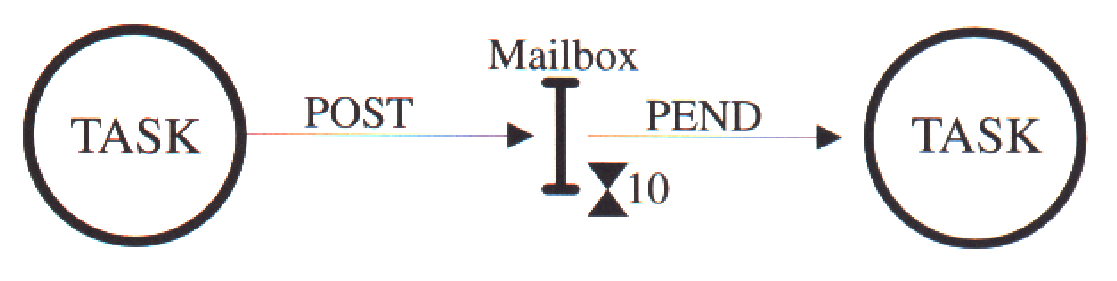
\includegraphics[width=12cm]{mailbox.png}
\end{center}

If a task wishes to receive a message coming from a void mailbox, it is suspended until the arrival of
the message, or during a lapse of time defined by the application. Each mailbox is thus associated to
a waiting list containing these suspended tasks. When the message is posted, it's the highest priority
waiting task that receives the message.

All information about the functions of \uCOSII~allowing the management of the mailboxes can be
found in the user's manual pp 32-43.

 Open the project \kw{Mailbox}.
 
This project contains two tasks :
\begin{itemize}
\item \kw{AppKeyboardTask} is the task which manages the keyboard: if a new key is pressed, the
\kw{KeyBuffer} variable contains the ASCII code of this key. The task is reactivated every 25ms to
detect the actions of the user. \kw{KeyboardScan()} is the function in charge of scanning the matrix
keyboard, it is defined in the file \kw{Keyboard.c}.
\item \kw{AppLCDTask} displays a character on the LCD screen. The function \kw{DispStr()} is defined in the
file \kw{LCD.c} containing all the functions pre-written for the LCD. You will find a short explanation
of these fonctions in the \kw{LCD.h} file.
\end{itemize}

\E{Create a mailbox allowing to transmit the characters pressed on the keyboard to the task displaying
the characters on the screen.
}{}
%\marginpar{OK add caption and refr to listing} done


\end{document}
